\documentclass{beamer}
%%% ========== Package setup ==========
\usepackage{xeCJK}      % Chinese words package
\usepackage{fontspec}   % Word fonts package
\usepackage{listings}   % Wrap Figure or table package
\usepackage{wrapfig}    % Multicolumn package
\usepackage{multicol}   % Multicolumn package
\usepackage{pdflscape}  % Landscpae package
\usepackage{hyperref}   % Hyperlink package
\usepackage{tikz}       % TikZ picture package(Docs: https://ftp.ntou.edu.tw/ctan/graphics/pgf/base/doc/pgfmanual.pdf)
\usepackage[backend=bibtex, style=ieee]{biblatex} % Biblatex reference package(Docs: https://distrib-coffee.ipsl.jussieu.fr/pub/mirrors/ctan/macros/latex/contrib/biblatex/doc/biblatex.pdf, Cheat Sheet: https://ftp.ntou.edu.tw/ctan/info/biblatex-cheatsheet/biblatex-cheatsheet.pdf)

\usepackage[outline]{contour} % glow around text
\usepackage{amsmath}
\usepackage{mathtools}

%%% ========== Slide setting ==========
%% Slide theme setup
\usetheme{CambridgeUS}
\usecolortheme{wolverine}

%% Setup chinese words encoder
\XeTeXlinebreaklocale "zh"
\XeTeXlinebreakskip = 0pt plus 1pt

%% More word fonts
\setmainfont{Times New Roman}
\renewcommand{\familydefault}{\rmdefault}
\setCJKmainfont{標楷體}

% Setting for figure and table numbering
\setbeamertemplate{caption}[numbered]

% TikZ setting
\usetikzlibrary{positioning}
\usetikzlibrary{calc}
\usetikzlibrary{arrows.meta}

% Biblatex setting
\addbibresource{refs.bib}
\ExecuteBibliographyOptions{eprint=false}
\ExecuteBibliographyOptions{url=false}

%%% ========== Title setup ==========
\date{June 9, 2022}
\title{Reinforcement learning for UAV attitude control}
\author{Wu, Po Hsun}
\institute[]{\emph{Department of Aerospace Engineering\\ Tamkang University}}
\logo{
\includegraphics[height=1.5cm]{figs/watermark_tku.eps}}

%%% ========== Document ==========
\begin{document}
    \maketitle

    % ---------- Contents ----------
    \section*{Contents}
    \begin{frame}
        \frametitle{\secname}

        \tableofcontents

    \end{frame}

    % ---------- Introduction ----------
    \section{Introduction}
    \begin{frame}
        \frametitle{\secname}

        \begin{itemize}
            \item[1.] What is Attitude Control?
            \item[2.] What is Reinforcement Learning?
        \end{itemize}

    \end{frame}

    \subsection*{What is Attitude Control?}
    \begin{frame}
        \frametitle{\subsecname}
        \begin{itemize}
            \item For Classical Control Theory
        \end{itemize}
        \vspace{1 pt}

        \begin{figure}
            \centering
            %%% ==================== CC_architecture ====================
% The figure of Classical Control architecture.
% Author: Wu, Po Hsun
% Date: May 28, 2022
%
\tikzstyle{circlenode}=[circle, draw=black, thick, minimum size=1mm]
\tikzstyle{squarednode}=[rectangle, draw=black, thick, minimum size=0mm, font=\footnotesize]

\begin{tikzpicture}[
    ->, >={latex},
    node distance=0.5cm,
    every state/.style={thick}
    ]
    % ---------- Nodes ----------figs/CC_architecture.tikz
    \node[]             (input)                                 {$r(t)$};
    \node[circlenode]   (sum)           [right=of input]        {};
    \node[squarednode]  (controller)    [right=of sum]          {Controller};
    \node[squarednode]  (plane)         [right=of controller]   {Plane};
    \node[]             (output)        [right=of plane]        {$y(t)$};

    % ---------- Lines ----------
    \draw[] (input.east) -- (sum.west);
    \draw[] (sum.east) -- (controller.west);
    \draw[] (controller.east) -- (plane.west);
    \draw[] ($(plane.east)+(0.2,0)$) -- ++(0,-1) -| ($(sum.south)$);
    \draw[] (plane.east) -- (output.west);

    % ---------- Symbols ----------
    \node[right] at ($(sum.south)+(0,-0.2)$)    {$-$};
    \node[above] at ($(sum.west)+(-0.2,0)$)     {$+$};
    \node[above] at ($(sum.east)+(0.2,0)$)      {$e(t)$};

    % ---------- Legend ----------
    \node[right, align=left] at (output.east) {
        $r(t)$: reference \\
        $y(t)$: state \\
        $e(t)$: error
    };

\end{tikzpicture}
            \caption{Block diagram for classical control}
        \end{figure}

    \end{frame}

    \subsection*{What is Reinforcement Learning?}
    \begin{frame}
        \frametitle{\subsecname}

        \begin{figure}
            \centering
            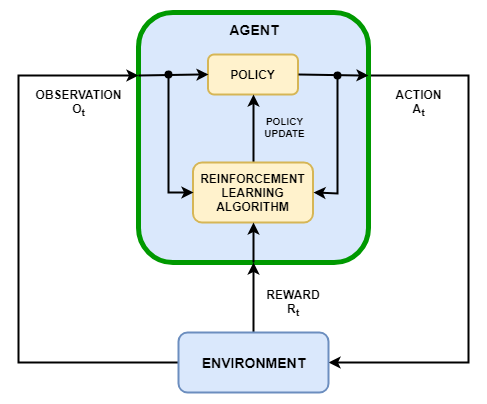
\includegraphics[scale=.3]{figs/RL_architecture.png}
            \caption{Reinforcement Learning architecture\cite{Flight_Controller_Synthesis_Via_Deep_Reinforcement_Learning}}
        \end{figure}

    \end{frame}

    \subsection*{Mix it together}
    \begin{frame}
        \frametitle{\subsecname}
        \begin{itemize}
            \item Apply reinforcement learning to control theory.
        \end{itemize}

        \begin{figure}
            \centering
            %%% ==================== RLC_architecture ====================
% The figure of Reinforcement Learning Controller architecture.
% Author: Wu, Po Hsun
% Date: May 28, 2022
%
\tikzstyle{circlenode}=[circle, draw=black, thick, minimum size=1mm]
\tikzstyle{squarednode}=[rectangle, draw=black, thick, minimum size=0mm, font=\footnotesize]

\begin{tikzpicture}[
    ->, >={latex},
    node distance=0.5cm,
    every state/.style={thick}
    ]
    % ---------- Nodes ----------
    \node[]             (input)                                 {$r(t)$};
    \node[circlenode]   (sum)           [right=of input]        {};
    \node[squarednode]  (controller)    [right=of sum]          {Neural Network};
    \node[squarednode]  (plane)         [right=of controller]     {Plane};
    \node[]             (output)        [right=of plane]        {$y(t)$};
    \node[squarednode]  (RL_algorithm)  [above=of controller]   {RL Algorithm};

    % ---------- Lines ----------
    \draw[] (input.east) -- (sum.west);
    \draw[] (sum.east) -- (controller.west);
    \draw[] (controller.east) -- (plane.west);
    \draw[] ($(plane.east)+(0.2,0)$) -- ++(0,-1) -| ($(sum.south)$);
    \draw[] (plane.east) -- (output.west);

    \draw[] (RL_algorithm.south) -- (controller.north);
    \draw[] (plane.north) |- (RL_algorithm.east);
    \draw[] ($(sum.east)+(0.2,0)$) |- (RL_algorithm.west);

    % ---------- Symbols ----------
    \node[right] at ($(sum.south)+(0,-0.2)$)            {$-$};
    \node[above] at ($(sum.west)+(-0.2,0)$)             {$+$};
    \node[above] at ($(RL_algorithm.east)+(0.8,0)$)     {$R(t)$};
    \node[above] at ($(RL_algorithm.west)+(-0.4,0)$)    {$e(t)$};

    % ---------- Legend ----------
    \node[right, align=left] at (output.east) {
        $r(t)$: reference \\
        $y(t)$: state \\
        $e(t)$: error \\
        $R(t)$: Reward
    };

\end{tikzpicture}
            \caption{Block diagram for Neural Network controller}
        \end{figure}

    \end{frame}

    % ---------- Paper Review ----------
    \section{Paper Review}
    \begin{frame}
        \frametitle{\secname}

        \begin{itemize}
            \item \fullcite{Flight_Controller_Synthesis_Via_Deep_Reinforcement_Learning}
                \begin{itemize}
                    \item[1.] Adding noise to the plane(or environment).
                    \item[2.] Using Gazebo as a physics simulator.
                \end{itemize}
            \item \fullcite{Reinforcement_Learning_for_UAV_Attitude_Control}
                \begin{itemize}
                    \item[1.] Provide a training framework.
                    \item[2.] Comparing some RL algorithm training results.
                \end{itemize}
        \end{itemize}

    \end{frame}

    % ---------- Reinforcement Learning ----------
    \section{Reinforcement Learning}
    \begin{frame}
        \frametitle{\secname}

        \begin{itemize}
            \item RL is a area of Mechine Learning.
            \item RL will interact with the environment.
            \item RL aims to achieve the maximum reward by changing the neural network parameters.
            %%% ==================== Argument maximum of reward ====================
% The equation of Argument maximum of reward.
% Author: Wu, Po Hsun
% Date: June 01, 2022
%
\begin{equation}
    \arg\max_{\theta}{\mathit{R(t)}}
    \label{eq:Argmax_reward}
\end{equation}
        \end{itemize}

        \begin{figure}
            \centering
            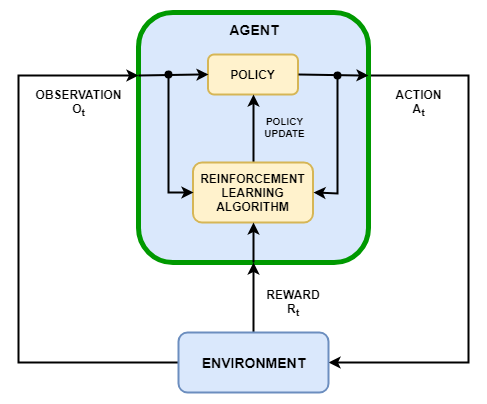
\includegraphics[scale=.2]{figs/RL_architecture.png}
            \caption{Reinforcement Learning architecture\cite{Flight_Controller_Synthesis_Via_Deep_Reinforcement_Learning}}
        \end{figure}

    \end{frame}

    \subsection*{Artificial Neural Network}
    \begin{frame}
        \frametitle{\subsecname}

        \begin{itemize}
            \item Artificial Neural Network is a nonlinear model.
            \item \eqref{eq:ANN_matrix} and \eqref{eq:ANN_variable} is the equations of Neural Network
        \end{itemize}

        %%% ==================== ANN matrix form ====================
% The equation of artificial neural network in matrix form.
% Author: Wu, Po Hsun
% Date: May 31, 2022
%
\begin{equation}
    \begin{bmatrix}
        a_{1}^{(1)} \\
        a_{2}^{(1)} \\
        \vdots \\
        a_{m}^{(1)}
    \end{bmatrix} = \sigma
    \begin{pmatrix}
        \color{black}
        \begin{bmatrix}
            w_{1,0} & w_{1,1} & \ldots & w_{1,n} \\
            w_{2,0} & w_{2,1} & \ldots & w_{2,n} \\
            \vdots  & \vdots  & \ddots & \vdots  \\
            w_{m,0} & w_{m,1} & \ldots & w_{m,n}
        \end{bmatrix}
        \begin{bmatrix}
            a_{1}^{(0)} \\
            a_{2}^{(0)} \\
            \vdots \\
            a_{n}^{(0)}
        \end{bmatrix} +
        \begin{bmatrix}
            b_{1}^{(0)} \\
            b_{2}^{(0)} \\
            \vdots \\
            b_{m}^{(0)}
        \end{bmatrix}
    \end{pmatrix}
    \label{eq:ANN_matrix}
\end{equation}


        %%% ==================== ANN variable form ====================
% The equation of artificial neural network in variable form.
% Author: Wu, Po Hsun
% Date: May 31, 2022
%
\begin{equation}
    {a^{(1)}} = \sigma \left(
        \mathbf{W}^{(0)} {a^{(0)}}+\mathbf{b}^{(0)}
    \right), \quad
    \begin{cases*}
        \mathbf{W} \in \mathbb{R}^{m\times n} \\
        \mathbf{a} \in \mathbb{R}^{n} \\
        \mathbf{b} \in \mathbb{R}^{m}
    \end{cases*}
    \label{eq:ANN_variable}
\end{equation}



    \end{frame}

    \begin{frame}
        \frametitle{\subsecname}

        \begin{figure}
            \centering
            \scalebox{.7}{%%% ==================== Artificial Neuro Network ====================
% The figure of Artificial Neuro Network architecture.
% Author: Izaak Neutelings
% Date: September 2021
% Reference: https://tikz.net/neural_networks/
%
\colorlet{myred}{red!80!black}
\colorlet{myblue}{blue!80!black}
\colorlet{mygreen}{green!60!black}
\colorlet{myorange}{orange!70!red!60!black}
\colorlet{mydarkred}{red!30!black}
\colorlet{mydarkblue}{blue!40!black}
\colorlet{mydarkgreen}{green!30!black}

\tikzstyle{node}=[thick,circle,draw=myblue,minimum size=22,inner sep=0.5,outer sep=0.6]
\tikzstyle{node in}=[node,green!20!black,draw=mygreen!30!black,fill=mygreen!25]
\tikzstyle{node hidden}=[node,blue!20!black,draw=myblue!30!black,fill=myblue!20]
\tikzstyle{connect}=[->, >={latex}, thick,mydarkblue] %,line cap=round


\begin{tikzpicture}[x=2.7cm,y=1.6cm]
    \message{^^JNeural network activation}
    \def\NI{5} % number of nodes in input layers
    \def\NO{4} % number of nodes in output layers
    \def\yshift{0.4} % shift last node for dots

    % INPUT LAYER
    \foreach \i [evaluate={\c=int(\i==\NI); \y=\NI/2-\i-\c*\yshift; \index=(\i<\NI?int(\i):"n");}] in {1,...,\NI}{ % loop over nodes
        \node[node in,outer sep=0.6] (NI-\i) at (0,\y) {$a_{\index}^{(0)}$};
    }

    % OUTPUT LAYER
    \foreach \i [evaluate={\c=int(\i==\NO); \y=\NO/2-\i-\c*\yshift; \index=(\i<\NO?int(\i):"m");}] in {\NO,...,1}{ % loop over nodes
        \ifnum\i=1 % high-lighted node
            \node[node hidden] (NO-\i) at (1,\y) {$\Sigma$};
            \node[node hidden] (NO-\i_active) at (1.5,\y) {$\sigma$};
            \node[node hidden] (NO-\i_output) at (2,\y) {$a_{\index}^{(1)}$};
            \foreach \j [evaluate={\index=(\j<\NI?int(\j):"n");}] in {1,...,\NI}{ % loop over nodes in previous layer
                \draw[connect,white,line width=1.2] (NI-\j) -- (NO-\i);
                \draw[connect] (NI-\j) -- (NO-\i)
                node[pos=0.50] {\contour{white}{$w_{1,\index}$}};
            }
            \draw[connect] (NO-\i) -- (NO-\i_active);
            \draw[connect] (NO-\i_active) -- (NO-\i_output);
        \else % other light-colored nodes
            \node[node,blue!20!black!80,draw=myblue!20,fill=myblue!5] (NO-\i) at (1,\y) {$\Sigma$};
            \node[node,blue!20!black!80,draw=myblue!20,fill=myblue!5] (NO-\i_active) at (1.5,\y) {$\sigma$};
            \node[node,blue!20!black!80,draw=myblue!20,fill=myblue!5] (NO-\i_output) at (2,\y) {$a_{\index}^{(1)}$};
            \foreach \j in {1,...,\NI}{ % loop over nodes in previous layer
                \draw[connect,myblue!20] (NI-\j) -- (NO-\i);
            }
            \draw[connect,myblue!20] (NO-\i) -- (NO-\i_active);
            \draw[connect,myblue!20] (NO-\i_active) -- (NO-\i_output);
        \fi
    }

    % DOTS
    \path (NI-\NI) --++ (0,0.9+\yshift) node[midway,scale=1.2] {$\vdots$};
    \path (NO-\NO) --++ (0,0.9+\yshift) node[midway,scale=1.2] {$\vdots$};
    \path (NO-\NO_active) --++ (0,0.9+\yshift) node[midway,scale=1.2] {$\vdots$};
    \path (NO-\NO_output) --++ (0,0.9+\yshift) node[midway,scale=1.2] {$\vdots$};
\end{tikzpicture}}
            \caption{Artificial Neural Network}
        \end{figure}

    \end{frame}

    \subsubsection*{Training target}
    \begin{frame}
        \frametitle{\subsubsecname}

        \begin{itemize}
            \item Target function:
                $$f(x)=x^2$$
            \item Database:
                \begin{itemize}
                    \item $x=\{0,1,\cdots,9\}$ adding noise with normal distribution($\mu=0, \sigma=0.2$).
                    \item 100 datas for each point(total 1,000 datas).
                \end{itemize}
            \item Configuration:
                \begin{itemize}
                    \item 2 hidden layer, each layer with 50 neuros.
                    \item Two different learning rate($\alpha=0.01, 0.001$).
                \end{itemize}

        \end{itemize}

    \end{frame}

    \subsubsection*{Training result}
    \begin{frame}
        \frametitle{\subsubsecname}
        \begin{itemize}
            \item Overfitting happend at $\alpha=0.01$.
        \end{itemize}

        \begin{figure}
            \centering
            \begin{multicols}{2}
                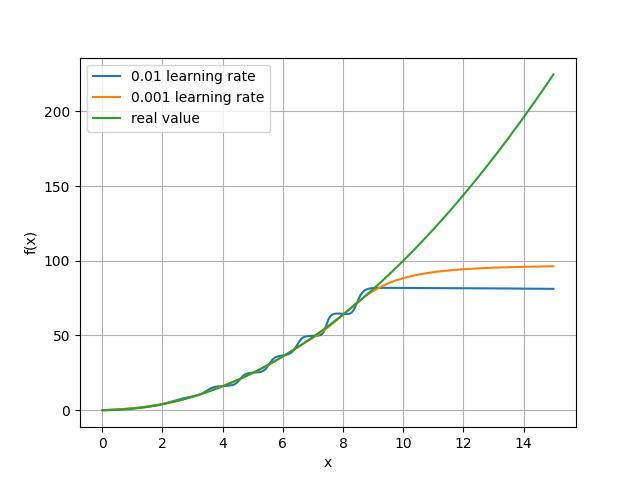
\includegraphics[width=2.2in]{figs/Value_50_2.jpg}
                \caption{$f(x)$ vs $x$}
                \columnbreak

                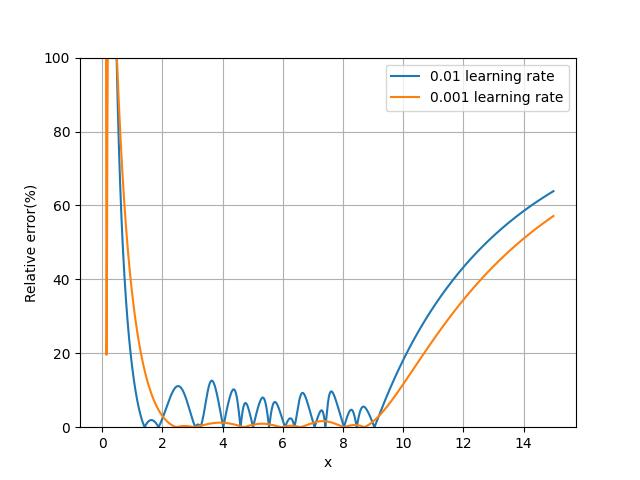
\includegraphics[width=2.2in]{figs/Error_50_2.jpg}
                \caption{Relative error}
            \end{multicols}
        \end{figure}
    \end{frame}

    \subsection*{Reinforcement Learning Algorithm}
    \begin{frame}
        \frametitle{\subsecname}
        \begin{itemize}
            \item Model-free:
                \begin{itemize}
                    \item[1.] Does not require a model of the environment.
                    \item[2.] It's an explicitly a trial-and-error method.
                \end{itemize}
            \item Model-base:
                \begin{itemize}
                    \item[1.] Require a model of the environment.
                    \item[2.] Will predict the future state.
                \end{itemize}
        \end{itemize}

    \end{frame}

    \subsubsection*{Q-learning}
    \begin{frame}
        \frametitle{\subsubsecname}
        \begin{itemize}
            \item Create a Q-table for each state and action.
            \item Find out the next action to maximizes the Q-value in the Q-table.
        \end{itemize}

        \begin{figure}
            \centering
            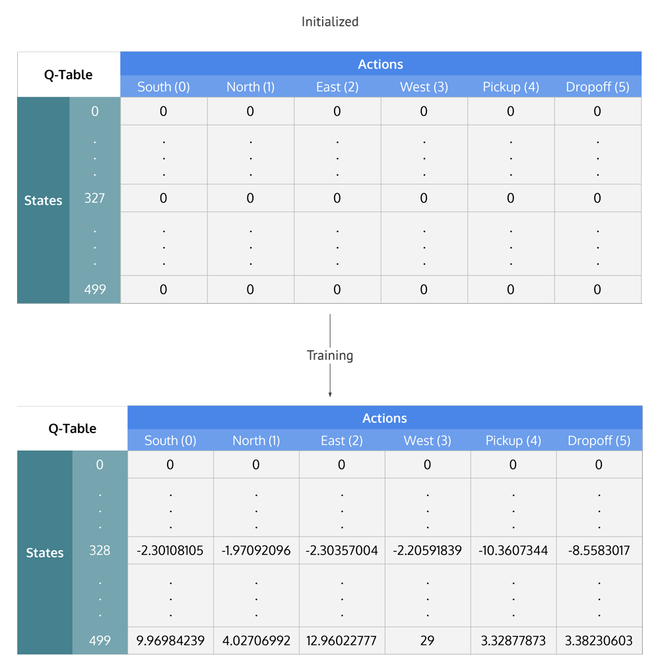
\includegraphics[scale=.2]{figs/Qtable.png}
            \caption{Q-table}
        \end{figure}

    \end{frame}

    \begin{frame}
        \frametitle{\subsubsecname}

        The iteration formula for Q-value
        $$Q^{new}(s_t, a_t) = Q(s_t, a_t) + \alpha(r_t + \gamma\max_{a}Q(s_{t+1}, a))$$
        The term $r_t$ is the current reward from the environment, and $\max\limits_{a}Q(s_{t+1}, a)$ is the maximum Q-value that can be obtain from next state $s_{t+1}$

    \end{frame}

    \begin{frame}
        \frametitle{\subsubsecname}
        \begin{figure}
            \centering
            %%% ==================== QLearning flow chart ====================
% The figure of Q-learning flow chart
% Author: Wu, Po Hsun
% Date: June 08, 2022
%
\tikzstyle{circlenode}=[circle, draw=black, thick, minimum size=1mm]
\tikzstyle{squarednode}=[rectangle, draw=black, thick, minimum size=0mm, font=\footnotesize]

\begin{tikzpicture}[
    ->, >={latex},
    node distance=0.5cm,
    every state/.style={thick}
    ]
    % ---------- Nodes ----------
    \node[squarednode]  (initialQtable)     []                         {Initialize Q-table};
    \node[squarednode]  (chooseAction)      [below=of initialQtable]   {Choose a action from Q-table};
    \node[squarednode]  (obtainState)       [below=of chooseAction]    {Obtain the state from the environment};
    \node[squarednode]  (measureReward)     [below=of obtainState]     {Measure the reward};
    \node[squarednode]  (updateQtable)      [below=of measureReward]   {Update Q-table};

    % ---------- Lines ----------
    \draw[] (initialQtable.south) -- (chooseAction.north);
    \draw[] (chooseAction.south) -- (obtainState.north);
    \draw[] (obtainState.south) -- (measureReward.north);
    \draw[] (measureReward.south) -- (updateQtable.north);
    \draw[] (updateQtable.south) |- ++(-3,-0.5) |- (chooseAction.west);

\end{tikzpicture}
            \caption{Q-learning flow chart}
        \end{figure}

    \end{frame}

    \begin{frame}
        \frametitle{\subsubsecname}
        \begin{figure}
            \centering
            %%% ==================== QLearning flow chart with NN ====================
% The figure of Q-learning flow chart with neural network
% Author: Wu, Po Hsun
% Date: June 08, 2022
%
\tikzstyle{circlenode}=[circle, draw=black, thick, minimum size=1mm]
\tikzstyle{squarednode}=[rectangle, draw=black, thick, minimum size=0mm, font=\footnotesize]

\begin{tikzpicture}[
    ->, >={latex},
    node distance=0.5cm,
    every state/.style={thick}
    ]
    % ---------- Nodes ----------
    \node[squarednode]  (initialQtable)     []                          {Initialize Q-table \& NN};
    \node[squarednode]  (chooseAction)      [below=of initialQtable]    {Choose a action from NN};
    \node[squarednode]  (obtainState)       [below=of chooseAction]     {Obtain the state from the environment};
    \node[squarednode]  (measureReward)     [below=of obtainState]      {Measure the reward};
    \node[squarednode]  (updateQtable)      [below=of measureReward]    {Update Q-table};
    \node[squarednode]  (trainNN)           [below=of updateQtable]     {Train the NN};

    % ---------- Lines ----------
    \draw[] (initialQtable.south) -- (chooseAction.north);
    \draw[] (chooseAction.south) -- (obtainState.north);
    \draw[] (obtainState.south) -- (measureReward.north);
    \draw[] (measureReward.south) -- (updateQtable.north);
    \draw[] (updateQtable.south) -- (trainNN.north);
    \draw[] (trainNN.south) |- ++(-3,-0.5) |- (chooseAction.west);

\end{tikzpicture}
            \caption{Q-learning flow chart using NN}
        \end{figure}

    \end{frame}

    % ---------- Ecpectation ----------
    \section{Expectation}
    \begin{frame}
        \frametitle{\secname}
        \begin{itemize}
            \item[1.] Realize on the inverse pendulum system.
            \item[2.] Realize on the fix wing UAV.
            \item[3.] Find more different algorithm.
        \end{itemize}

    \end{frame}

    % ---------- Q&A ----------
    \section{Q\&A}
    \begin{frame}

        \centering
        \Large Q\&A

    \end{frame}

    % ---------- References ----------
    \section*{References}
    \begin{frame}
        \frametitle{\secname}

        \printbibliography

    \end{frame}


\end{document}